\section{Geometrical classifiers} \ \label{geometrical_classifiers}

\subsection{Minimum Volume Enclosing Figure array classifier}

The construction of a classifier using array of identifiers is pretty simple and straightforward. The array is filled with minimum volume enclosing figures, one for each class in the training dataset. Every unknown pattern, sent for classification, moves through those figures and gets the information whether it lies inside the figure or not. In case of being part of identifier's interior the value given by the inclusion-equation (for ellipsoid see Equation \ref{eq:ellipsoid_affiliation}) is taken into consideration, which tells about the position inside the figure (where value 0 means that the point is in the figure's centre and 1 means that it lies on the surface). Finally, after all figures are checked, the one with the smallest equation value (and for which the point lies inside it), designates the class to which this unknown pattern should be classified to. If no figure accepts the point, it is rejected and treated as a foreign element. 

\begin{figure}[htp]
	\centering
	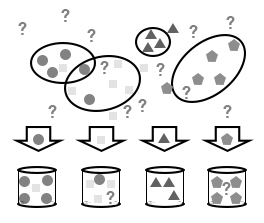
\includegraphics[width=0.75\textwidth]{Figures/ellipsoid_classification.jpg}
	\caption{ Array of ellipsoids that works as a classifier with rejection capabilities. Elements outside of existing ellipsoids are treated as a foreign patterns. Those within ellipsoids are classified as native patterns. }
	\label{fig:ellipsoids_array}\vspace{-3pt}
\end{figure}

\subsection{Optimizing figure size} \ \label{size_optimizing}

One way of increasing rejection ratio would be to decrease figure size. The smaller the volume the fewer points lie inside, which in return boosts rejection rates but worsens classification. Changing figure's size can be helpful in a situation in which two classes overlap and rejection of the elements is more desired result than misclassification. Another thing worth noting when using minimum volume enclosing figures is that their size can often be artificially enlarged by having at least one point that is located very far away from all other points in the same class. This situation can lead to decrease in rejection option rates as well as bigger misclassification between native elements' classes. Of course decreasing figure's size can result in the opposite situation. The key to deal with this difficulty is to find balance between decreasing figure's size and still getting high rejection and classification rates. Two approaches are proposed in this paper.

\subsubsection{Tolerance parameter manipulation}

The tolerance parameter, also denoted as $\varepsilon$ in Equation (\ref{eq:ellipsoid_affiliation}), can be used during point affiliation check-up to manipulate the result of the equation. By decreasing its value the figure ``shrinks`` evenly in all directions, and by increasing it more points are accepted as if they were lying inside the figure. In other words, by checking the distance of the point in regards to the minimum volume enclosing figure centre, the tolerance parameter can be used to ``decrease`` or ``increase`` the value resulting in acceptance or rejection.

Overall 100 tests there were performed with $\varepsilon$ consecutive values being~$(1, 0.98, 0.96, \dots, -0.98)$. Some of the charts presented in this section have been cropped in order to present only important data and preserve paper space, e.g. Figure \ref{fig:shrinking_ellipsoids_tolerance_manipulation} contains information only for $\varepsilon$ values from range $[-1, -0.56]$ because other values showed very poor classification and rejection rates thus there was no point in presenting them.

The results can be seen in Figure \ref{fig:shrinking_ellipsoids_tolerance_manipulation} and Figure \ref{fig:shrinking_rectangles_tolerance_manipulation}. Classification value corresponds to the number of native elements from the tested class that were correctly classified. Identification informs about number of native elements that were correctly classified (identified) by the ellipsoid, not necessarily to the proper class. Rejection value informs about correctly rejected foreign patterns. It's worth noting that when value of $\varepsilon$ becomes lesser than zero (which means that the figure shrinks in regards to its initial, unaltered size) there's a sudden drop in classification and identification rates. This could possibly be explained by the fact that many points lie on the surface of the minimum volume enclosing figure and get rejected after reducing its size. This is expected behaviour because minimum volume enclosing figures are somewhat unfolded on points they are trained on during creation process.

When testing hyper rectangles with gradually decreasing $\varepsilon$ values the results are very weak as opposed to the ellipsoid ones. The main disadvantage of this solution is the sudden drop in identification and rejection rates when having values of $\varepsilon$ lesser than zero.

\begin{figure}[htp]
	\centering
	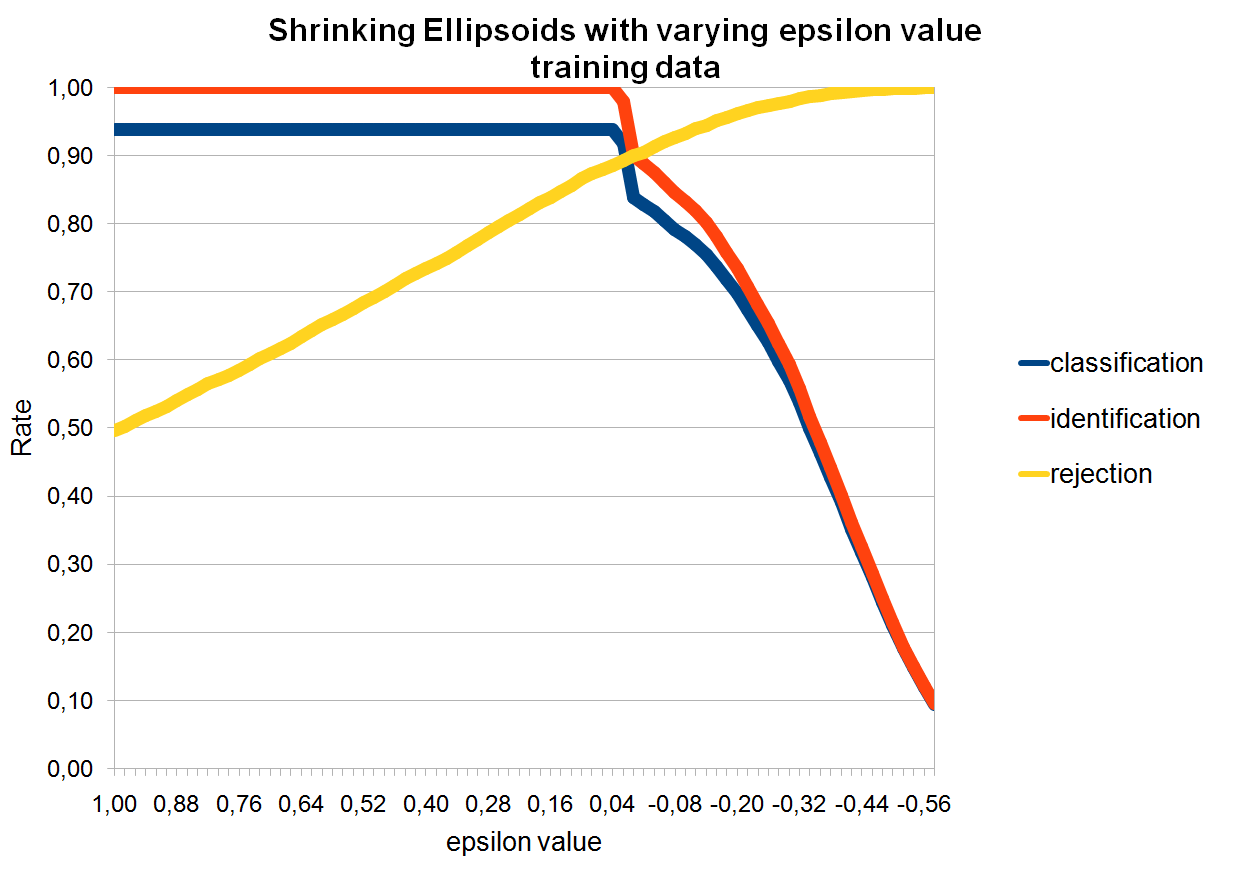
\includegraphics[width=0.80\textwidth]{Figures/charts/DIGITS/DIGITS_ShrinkingEllipsoidsToleranceTraining.png}
	\hspace{12pt}
	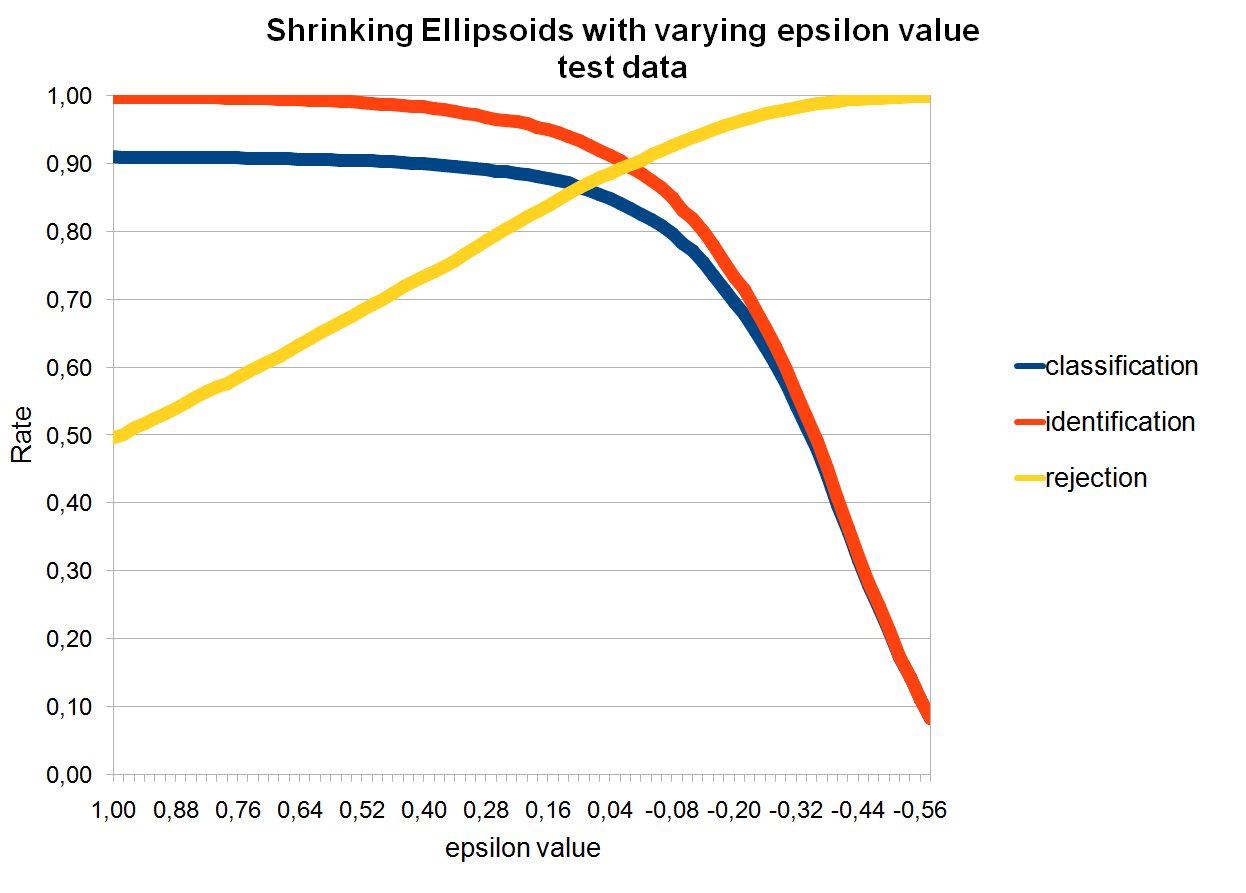
\includegraphics[width=0.80\textwidth]{Figures/charts/DIGITS/DIGITS_ShrinkingEllipsoidsToleranceTest.png}
	\caption{ Classification, identification and rejection rates for different $\varepsilon$ values for ellipsoids. Classification value corresponds to the number of native elements from the tested class that were correctly classified. Identification informs about number of native elements that were correctly classified (identified) by the ellipsoid, not necessarily to the proper class. Rejection value informs about correctly rejected foreign patterns. The bigger the values, the better. }
	\label{fig:shrinking_ellipsoids_tolerance_manipulation}\vspace{-3pt}
\end{figure}

\begin{figure}[htp]
\centering
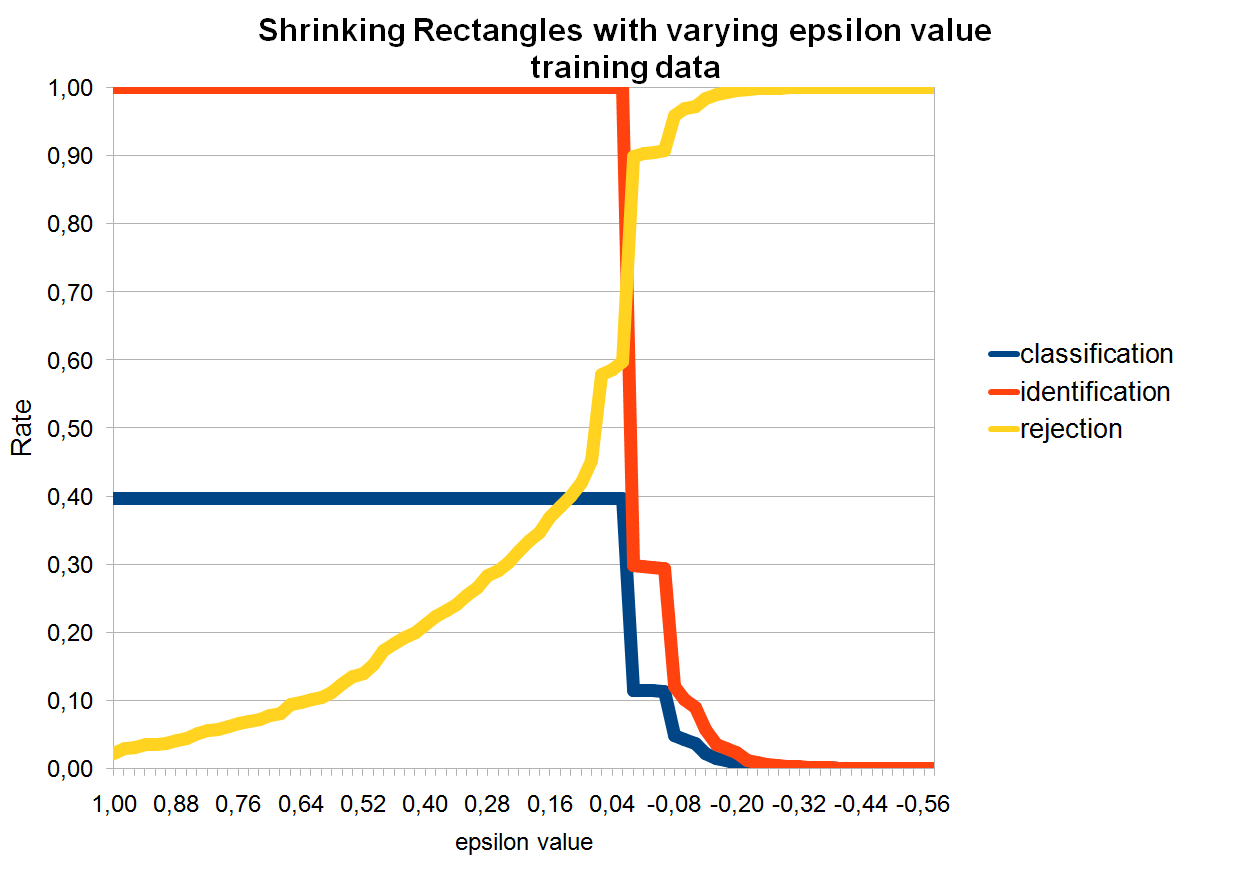
\includegraphics[width=0.80\textwidth]{Figures/charts/DIGITS/DIGITS_ShrinkingRectanglesToleranceTraining.png}
\hspace{12pt}
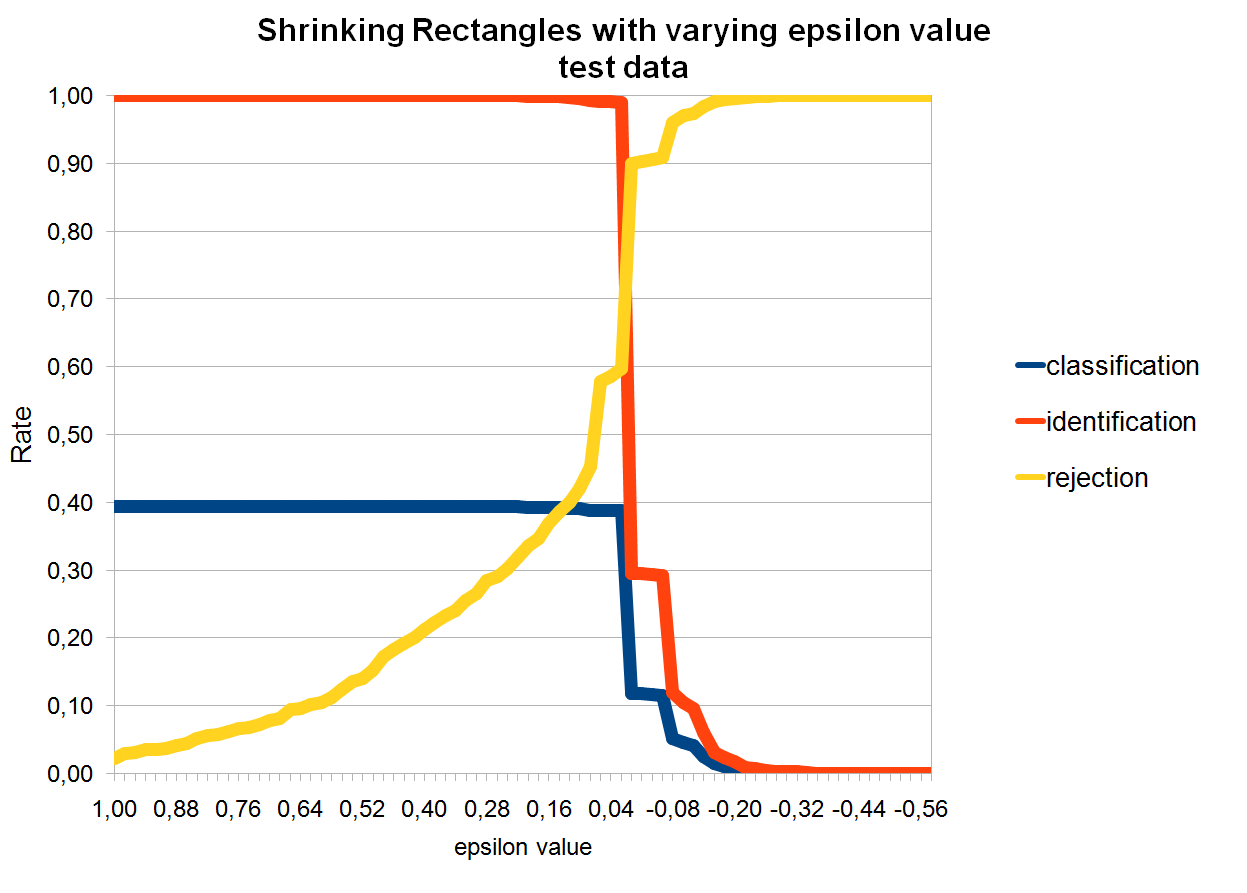
\includegraphics[width=0.80\textwidth]{Figures/charts/DIGITS/DIGITS_ShrinkingRectanglesToleranceTest.png}
\caption{ Classification, identification and rejection rates for different $\varepsilon$ values for hyper rectangles. Classification value corresponds to the number of native elements from the tested class that were correctly classified. Identification informs about number of native elements that were correctly classified (identified) by the ellipsoid, not necessarily to the proper class. Rejection value informs about correctly rejected foreign patterns. The bigger the values, the better. }
\label{fig:shrinking_rectangles_tolerance_manipulation}\vspace{-3pt}
\end{figure}

\subsubsection{Native elements removal}

The main problem connected to manipulating the tolerance parameter is the fact that the shape of the figure stays the same for the whole time. This is not a desired solution in a situation in which some of the patterns are located far from the rest of native elements in the same class, which results in a creation of very big figure that is mostly empty inside. In such case it theoretically should be better to ignore such points and prefer smaller volume figure with a slightly worse classification capabilities. This approach has been tested by checking classification and rejection rates for ellipsoids and hyper rectangles built on increasingly smaller datasets. Each step of the shrinking figure algorithm consists of creating a figure for a certain number of patterns. Those elements are sorted based on the inclusion testing function value (for example Equation \ref{eq:ellipsoid_affiliation} or Algorithm \ref{eq:rectangle_affiliation}), and 5 most distant ones are removed from the set. The classification and rejection rates are obtained based on the new figure created on this smaller set and the whole procedure is repeated. The results of this algorithm, which can be seen in Figure \ref{fig:shrinking_ellipsoids_elements_rejection} and Figure \ref{fig:shrinking_rectangles_elements_rejection}, were obtained for 80 steps which resulted (in the 80th step) in 395 elements removed from the original data set while using $\varepsilon$ value equal 0.

\begin{figure}[htp]
	\centering
	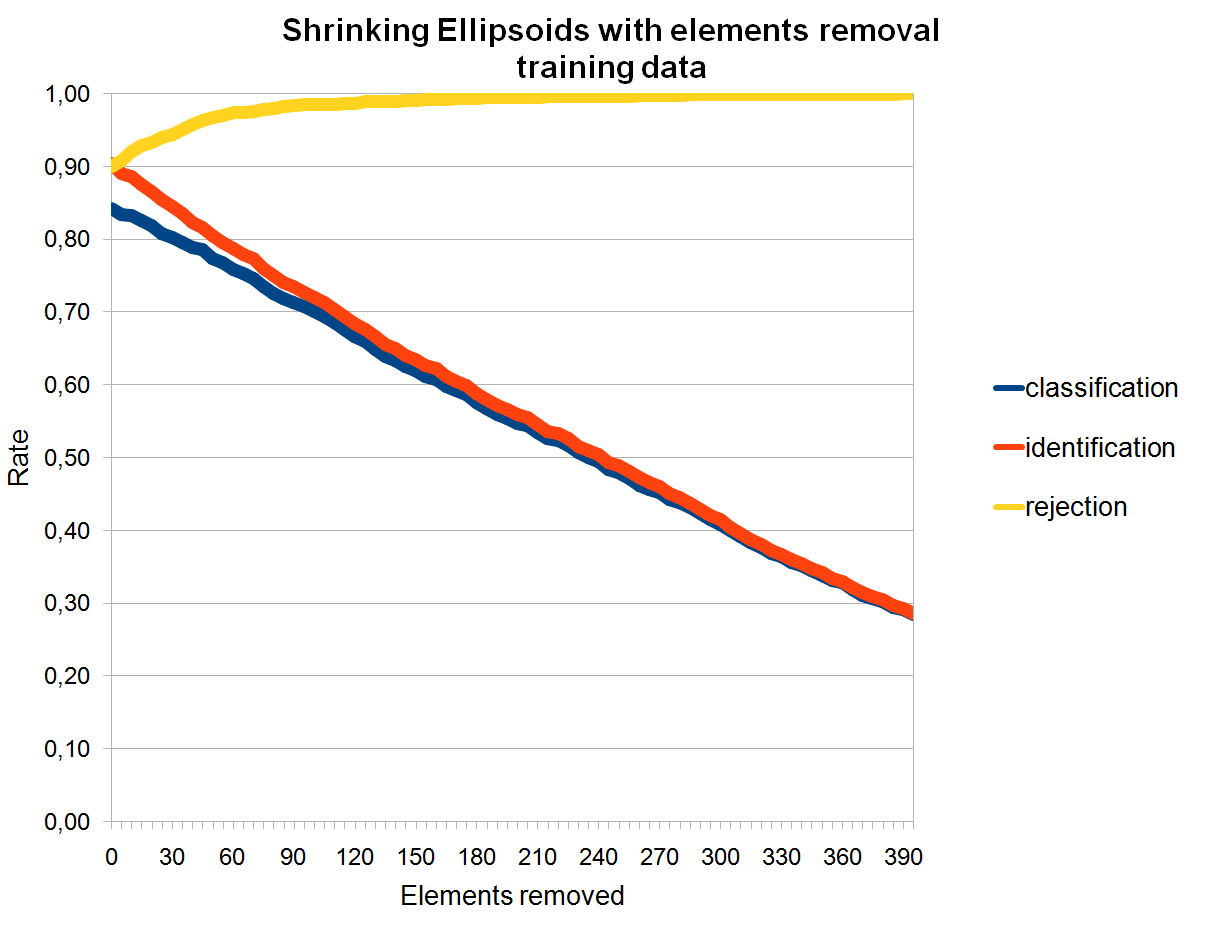
\includegraphics[width=0.80\textwidth]{Figures/charts/DIGITS/DIGITS_ShrinkingEllipsoidsElementsRemovalTraining.png}
	\hspace{12pt}
	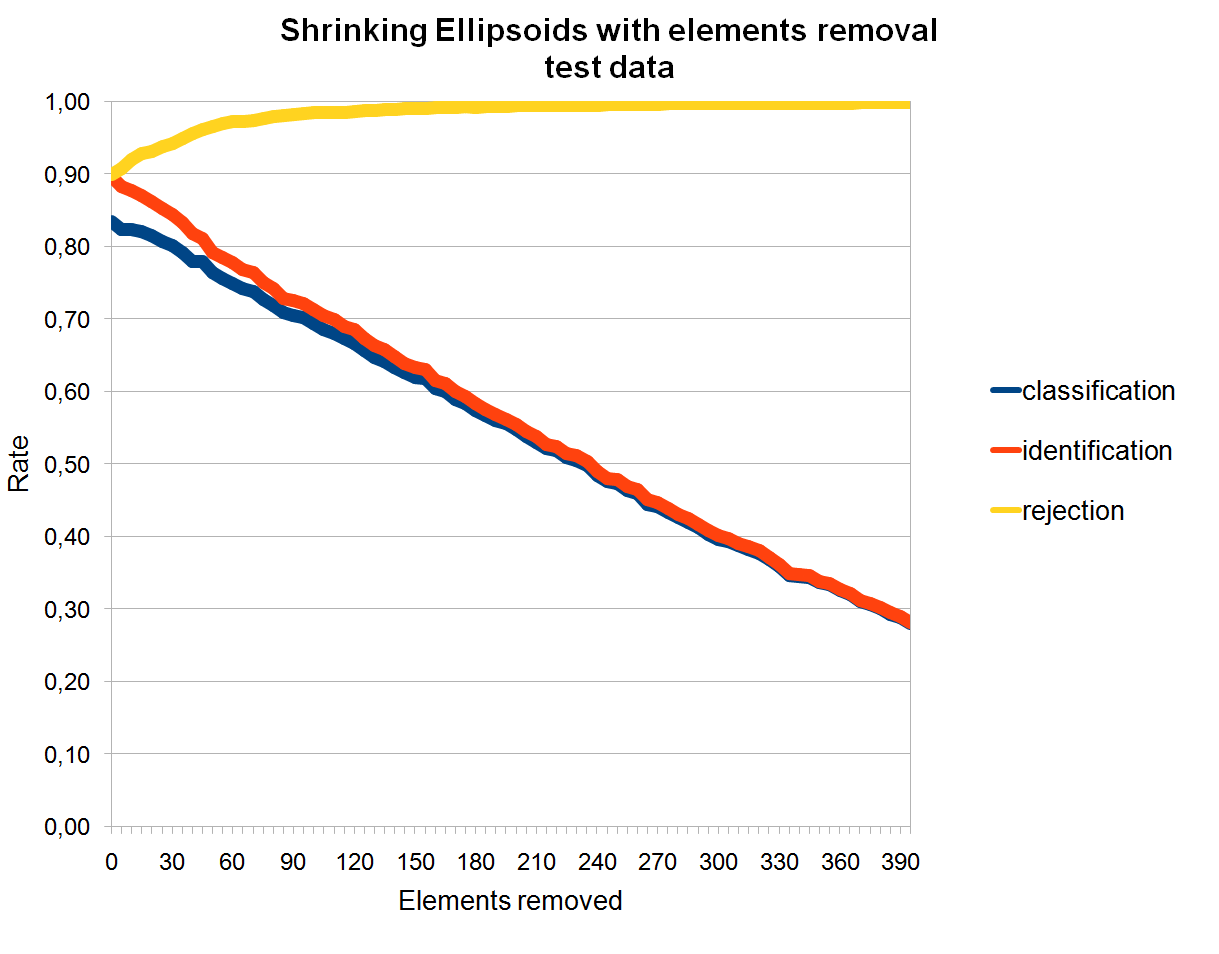
\includegraphics[width=0.80\textwidth]{Figures/charts/DIGITS/DIGITS_ShrinkingEllipsoidsElementsRemovalTest.png}
	\caption{ Classification, identification and rejection rates for each native element removal step while using ellipsoids. In each step 5 elements were deleted from the set resulting in overall 390 elements removed in the final 80th step. Classification value corresponds to the number of native elements from the tested class that were correctly classified. Identification informs about number of native elements that were correctly classified (identified) by the ellipsoid, not necessarily to the proper class. Rejection value informs about correctly rejected foreign patterns. The bigger the values, the better. }
	\label{fig:shrinking_ellipsoids_elements_rejection}\vspace{-3pt}
\end{figure}

\begin{figure}[htp]
	\centering
	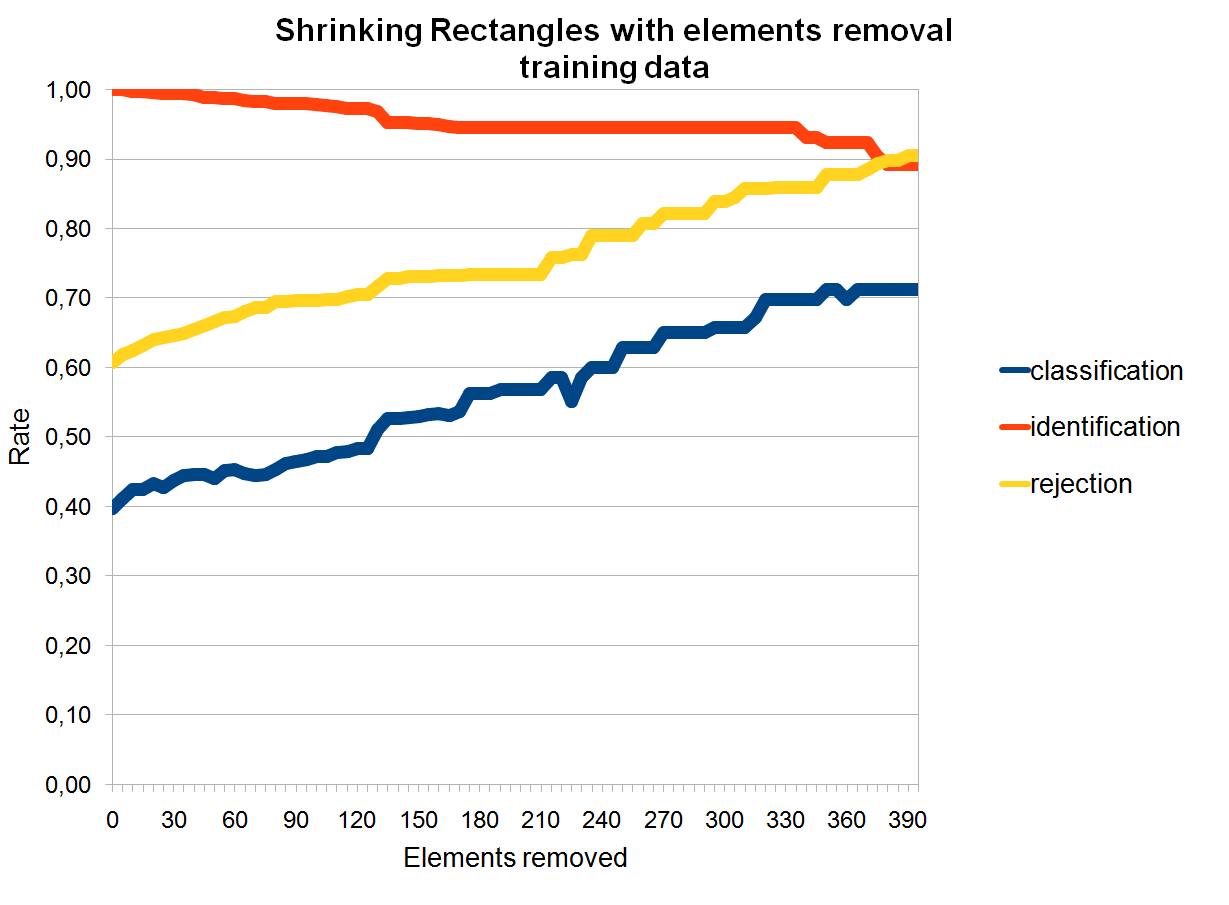
\includegraphics[width=0.80\textwidth]{Figures/charts/DIGITS/DIGITS_ShrinkingRectanglesElementsRemovalTraining.png}
	\hspace{12pt}
	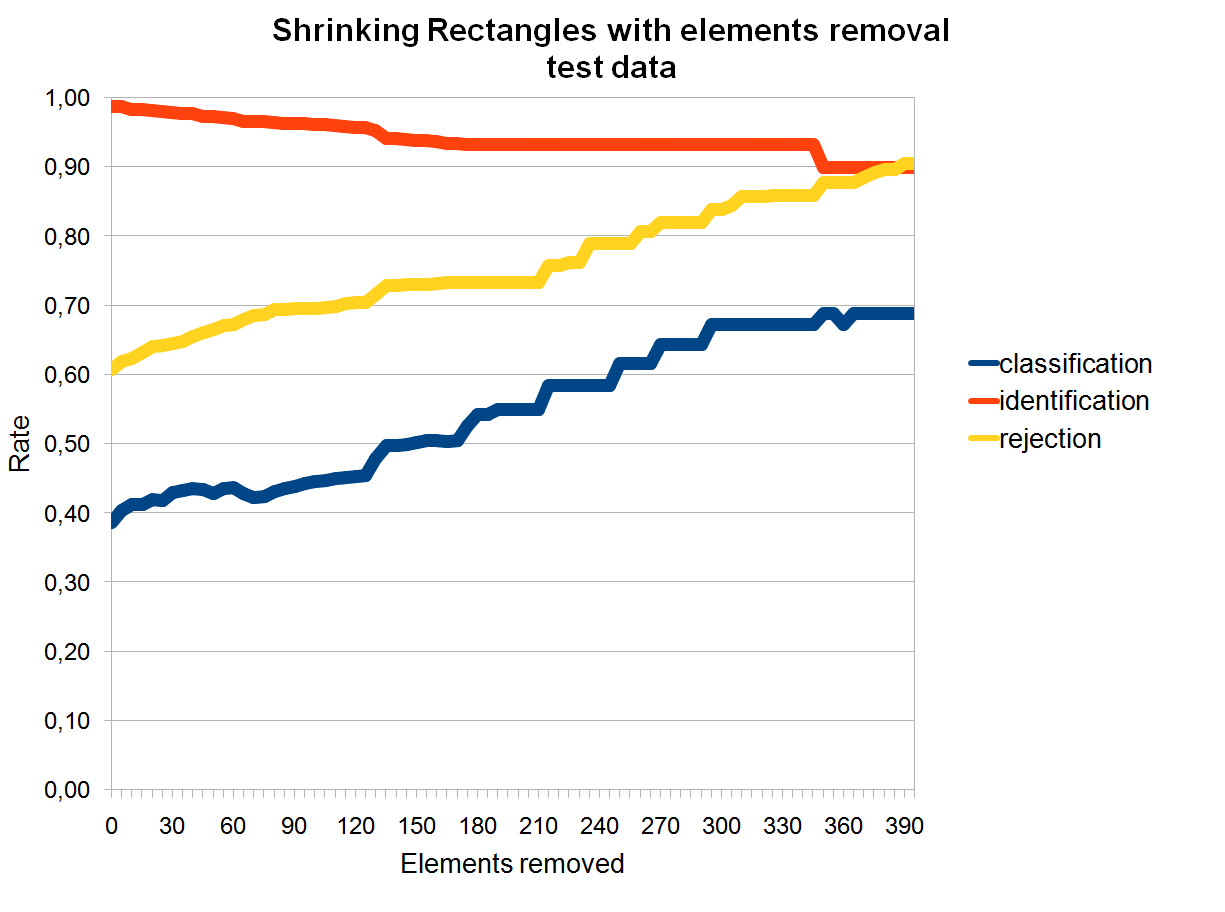
\includegraphics[width=0.80\textwidth]{Figures/charts/DIGITS/DIGITS_ShrinkingRectanglesElementsRemovalTest.png}
	\caption{ Classification, identification and rejection rates for each native element removal step while using hyper rectangles. In each step 5 elements were deleted from the set resulting in overall 390 elements removed in the final 80th step. Classification value corresponds to the number of native elements from the tested class that were correctly classified. Identification informs about number of native elements that were correctly classified (identified) by the ellipsoid, not necessarily to the proper class. Rejection value informs about correctly rejected foreign patterns. The bigger the values, the better. }
	\label{fig:shrinking_rectangles_elements_rejection}\vspace{-3pt}
\end{figure}

\subsection{Summary}

The tests performed on the classifier using array of identifiers prove that it can successfully combine classification and rejection tasks. While being unable to do the multi-class classification on their own, combined ellipsoids can be very accurate at classification and rejecting foreigners. Minimum volume enclosing ellipsoids combine advantages of commonly used classifiers described in Chapter \ref{common_classifiers} such as easy point inclusion detection, and iterative construction algorithm that uses tolerance parameter for its stop condition. The main disadvantage of ellipsoid, and minimum volume enclosing figures in general, is the fact that it does not transform the feature space of presented data. In order to get good results the data should be separable, and no generalisation of information is done at all. This is completely different from the attitude introduced in random forest or svm.

Moreover, according to the tests described and performed in previous Subsection regarding figure size manipulations, some initial conclusions can be drawn. At first glance it seems that neither approach based on elements removal, nor $\varepsilon$ value manipulation showed results that would justify any data changes, as all tested modifications achieved highest scores using minimum volume enclosing figures constructed on unaltered training set, with $\varepsilon$ value set to 0. However it turns out that those conclusions are not necessarily justified as it is possible that some different datasets can actually benefit from size manipulations (see Section \ref{additional_tests}).